\documentclass[aspectratio=169]{beamer}
\mode<presentation>

\usepackage{adjustbox}
\usepackage{array}
\usepackage{fancyvrb}
\usepackage{relsize}
\usepackage{graphicx}
\usepackage[overlay,absolute]{textpos}
\usepackage{xcolor}

\usepackage{tikz}
\usetikzlibrary{arrows.meta}
\usetikzlibrary{positioning}
\usetikzlibrary{shapes.multipart}
\usetikzlibrary{shadows}
\usetikzlibrary{tikzmark}

\graphicspath{{../images}}

\usepackage{fontspec}
\setsansfont{Helvetica Neue Light}[
    BoldFont={Helvetica Neue Bold},
    BoldItalicFont={Helvetica Neue Bold Italic},
    ItalicFont={Helvetica Neue Light Italic}
]
\setmonofont{Iosevka Term}
\newfontface\helvreg{Helvetica Neue}

\definecolor{grayish}{gray}{0.8}

\title{Stack graphs}
\subtitle{Name resolution at scale}
\author{
    Douglas A. Creager
    \\
    Hendrik van~Antwerpen
}
\institute{
\includegraphics[width=2.5em]{github-mark.pdf}\vspace{2em}}
\date{Eelco Visser Commemorative Symposium\\\textsmaller[1]{April 5, 2023 – TU Delft}}

\setbeamercolor{title}{fg=black}
\setbeamerfont{title}{series=\bfseries,size=\larger[1]}
\setbeamerfont{subtitle}{series=\mdseries,size=\smaller[2]}
\setbeamerfont{author}{size=\smaller[1]}
\setbeamerfont{institute}{size=\normalsize}
\setbeamertemplate{navigation symbols}{}
\setbeamercolor{frametitle}{fg=black}
\setbeamerfont{frametitle}{series=\bfseries}

% Picture credits

\makeatletter
\def\picturecredits{}
\newcommand{\picturecredit}[4]{
    \protected@xappto\picturecredits{
        \textsmaller[3]{Slide \theframenumber} &
        \textsmaller[2]{#1, “#2”} \vspace*{-0.4em} \newline
        \textsmaller[3]{#3, \url{#4}} \\
    }
}
\makeatother

\newlength{\titlewidth}
\newcommand{\flattitle}[3]{
    \settowidth{\titlewidth}{\textbf{\LARGE #3}}
    \begin{textblock*}{\titlewidth}(#1,#2)
        \textbf{\LARGE #3}
    \end{textblock*}
}
\newcommand{\shadowedtitle}[3]{
    \settowidth{\titlewidth}{\textbf{\LARGE #3}}
    \addtolength{\titlewidth}{0.5mm}
    \begin{textblock*}{\titlewidth}(#1+0.4mm,#2+0.4mm)
        \textbf{\LARGE #3}
    \end{textblock*}
    \begin{textblock*}{\titlewidth}(#1,#2)
        \textbf{\textcolor{white}{\LARGE #3}}
    \end{textblock*}
}

\usepackage[outputdir=.build]{minted}
\usemintedstyle{colorful}
\setminted{autogobble,fontsize=\relscale{0.8},frame=single,framesep=6pt,escapeinside=??}

%%%%%%%%%%%%%%%%%%%%%%%%%%%%%%%%%%%%%%%%%%%%%%%%%%%%%%%%%%%%%%%%%%%%%%%%%%%%%%%%
% tikz stuff

\makeatletter
\tikzset{tikzmark suffix=-\theframenumber-\the\beamer@slideinframe}
\makeatother

\tikzset{binding arrow/.style={->, red, thick, -{Triangle[]}}}

\newcommand{\codeline}[3][]{%
    \tikz[remember picture] \draw [overlay, binding arrow, #1] (#2) -- (#3);%
}

\newcommand{\curvecodeline}[4][]{%
    \tikz[remember picture] \draw [overlay, binding arrow, #1] (#2) .. controls #3 .. (#4);%
}

\newcommand{\highlightdef}[1]{%
    \tikz[remember picture]
      \draw [overlay, draw=none, fill=red!25]
        ([xshift=-1pt, yshift=8pt] pic cs:#1_start)
        rectangle
        ([xshift=1pt, yshift=-2pt] pic cs:#1_end)
        ;%
}

\newcommand{\highlightboth}[1]{%
    \tikz[remember picture]
      \draw [overlay, draw=brown, thin, fill=yellow!25]
        ([xshift=-1pt, yshift=8pt] pic cs:#1_start)
        rectangle
        ([xshift=1pt, yshift=-2pt] pic cs:#1_end)
        ;%
}

\newcommand{\highlightref}[1]{%
    \tikz[remember picture]
      \draw [overlay, draw=none, fill=blue!25]
        ([xshift=-1pt, yshift=8pt] pic cs:#1_start)
        rectangle
        ([xshift=1pt, yshift=-2pt] pic cs:#1_end)
        ;
}

%%%%%%%%%%%%%%%%%%%%%%%%%%%%%%%%%%%%%%%%%%%%%%%%%%%%%%%%%%%%%%%%%%%%%%%%%%%%%%%%
% stack graph stuff

\newlength{\scopegap}
\setlength{\scopegap}{0.9cm}

\newcommand\scoped[2]{#1 \lfloor #2 \rfloor}
\newcommand\nilsymbolstack{\mathit{\diamond}}
\newcommand\nilscopestack{\mathit{\circ}}

\newcommand\PushSymbol[1]{$\mathit{\textrm{\raisebox{0.05em}{\scriptsize $\downarrow$}} \; \texttt{#1}}$}
\newcommand\PushScopedSymbol[2]{$\mathit{\textrm{\raisebox{0.05em}{\scriptsize $\downarrow$}} \; \scoped{\texttt{#1}}{#2}}$}
\newcommand\PopSymbol[1]{$\mathit{\textrm{\raisebox{0.05em}{\scriptsize $\uparrow$}} \; \texttt{#1}}$}
\newcommand\PopScopedSymbol[1]{$\mathit{\textrm{\raisebox{0.05em}{\scriptsize $\uparrow$}} \; \scoped{\texttt{#1}}{\bullet}}$}

\definecolor{sgdef}  {RGB}{159,0,0}
\definecolor{sgpop}  {RGB}{230,142,131}
\definecolor{sgref}  {RGB}{0,112,196}
\definecolor{sgpush} {RGB}{161,190,230}
\definecolor{sgjump} {RGB}{161,64,140}

\newcommand\scopestackelement[1]{\textsf{\textcolor{sgjump}{#1}}}

\tikzset{root node/.style={
    node distance=0.5cm,
    circle, fill=black, inner sep=0pt,
    minimum size=0.35cm
}}

\tikzset{anon scope/.style={
    node distance=0.5cm,
    circle, fill=white, inner sep=0pt,
    draw=black, semithick,
    minimum size=0.35cm
}}

\tikzset{named scope/.style={
    node distance=0.5cm,
    circle, fill=white,
    draw=black, thick, node font={\smaller[2]},
    minimum size=0.35cm
}}

\tikzset{exported scope/.style={
    node distance=0.5cm,
    circle, fill=white,
    draw=sgjump, thick, text=sgjump, node font={\smaller[2]},
    minimum size=0.35cm
}}

\tikzset{symbol text/.style={
    fill=white,
    text height=1.5ex, text depth=0.25ex, node font={\ttfamily \relscale{0.8}},
    inner xsep=7pt,
    minimum size=0.75cm,
}}

\tikzset{definition/.style={
    node distance=0.5cm,
    draw=sgdef, thick,
    text=sgdef, symbol text,
}}

\tikzset{pop/.style={
    node distance=0.5cm,
    rectangle split,
    rectangle split parts=2,
    rectangle split horizontal,
    rectangle split draw splits=false,
    rectangle split ignore empty parts,
    draw=sgpop, thick, densely dashed,
    text=sgpop, symbol text,
}}
\newcommand{\popscope}{
    \nodepart{two}
    \hspace{-12pt}
    \tikz \node [circle, fill=sgjump, inner sep=0pt, minimum size=0.25cm] {};
}

\tikzset{reference/.style={
    node distance=0.5cm,
    draw=sgref, thick,
    text=sgref, symbol text,
}}

\tikzset{push/.style={
    node distance=0.5cm,
    rectangle split,
    rectangle split parts=2,
    rectangle split horizontal,
    rectangle split draw splits=false,
    rectangle split ignore empty parts,
    draw=sgpush, thick, densely dashed,
    text=sgpush, symbol text,
}}
\newcommand{\pushscope}[1]{
    \nodepart{two}
    \hspace{-12pt}
    \tikz \node [
        circle, fill=white,
        draw=sgjump,
        text=sgjump, inner sep=2pt,
        minimum size=0.25cm
    ] {\tiny #1};
}

\tikzset{control node/.style={
    node distance=0.5cm,
    draw=sgjump, thick,
    fill=white,
    text=sgjump,
    inner xsep=7pt, inner ysep=5pt,
    node font={\sffamily \smaller[1]},
}}

\newcommand{\widestsymbol}{}
\newcommand{\setwidestsymbol}[1]{\renewcommand{\widestsymbol}{#1}}
\newcommand{\sized}[2][\widestsymbol]{\makebox[\widthof{#1}]{#2}}

\tikzset{
  alt/.code args={<#1>#2#3}{%
    \alt<#1>{\pgfkeysalso{#2}}{\pgfkeysalso{#3}} % \pgfkeysalso doesn't change the path
  }
}

\tikzset{
    highlight node/.style={
        general shadow={fill=black, opacity=0.3},
        shadow scale=1, shadow xshift=2pt, shadow yshift=-2pt
    }
}
\tikzset{
    highlight node on/.code args={<#1>}{%
        \alt<#1>{\pgfkeysalso{highlight node}}{}%
    }
}

\tikzset{
    invisible/.style={opacity=0},
    visible on/.code args={<#1>}{%
        \alt<#1>{}{\pgfkeysalso{invisible}}%
    }
}

% Animating paths in a stack graph picture
%   Just add [highlighted on=<slide>] to an edge's style.  The line of the edge
%   will be blue and extra thick on <slide> AND ALL LATER SLIDES.  It will have
%   an arrowhead on SLIDE.
%
%   Together, this means that you add this to all of the edges that comprise a
%   path, with increasing <slide> values for each one, and beamer will create an
%   overlay animation showing the edges of the path get highlighted in order
%   each time you advance to the next slide.
\tikzset{highlight edge/.style={line width=2pt, blue, -}}
\tikzset{highlight edge frontier/.style={-{Triangle[length=4pt,width=4pt]}}}
\tikzset{
    show path on/.code args={<#1>}{%
        \alt<#1- >{\pgfkeysalso{highlight edge}}{}%
        \alt<#1  >{\pgfkeysalso{highlight edge frontier}}{}%
    }
}

\tikzset{
    highlight inner edge on/.code args={<#1>}{%
        \alt<#1>{\pgfkeysalso{highlight edge}}{}%
    }
}
\tikzset{
    highlight end edge on/.code args={<#1>}{%
        \alt<#1>{\pgfkeysalso{highlight edge, highlight edge frontier}}{}%
    }
}

\newlength\stwlength
\newcommand\makesamewidth[3][c]{%
  \settowidth{\stwlength}{#2}%
  \makebox[\stwlength][#1]{#3}%
}

\newcommand{\symbolstack}[1]{\langle \texttt{\relscale{0.8}#1} \rangle}

\newcommand{\scopestack}[1]{( \textsf{\relscale{0.8}#1} )}

\newcommand{\partialpath}[4]{%
    $\{#1\}$
    \hspace{0.01em}
    \scalebox{0.75}{\tikz[baseline={([yshift=-0.7ex] current bounding box.center)}] #2;}
    \texttt{\relscale{0.8}\textasciitilde\textasciitilde>}  % all that just to get a ~~> ligature
    \scalebox{0.75}{\tikz[baseline={([yshift=-0.7ex] current bounding box.center)}] #3;}
    \hspace{0.01em}
    $\{#4\}$
}

%%%%%%%%%%%%%%%%%%%%%%%%%%%%%%%%%%%%%%%%%%%%%%%%%%%%%%%%%%%%%%%%%%%%%%%%%%%%%%%%

\begin{document}

\begin{frame}
    \titlepage
\end{frame}


\section{Code Navigation}

\begin{frame}
    \begin{textblock*}{160mm}(0mm,0mm)
        \picturecredit{Ivan Radic}{Close-up of a compass graffiti on the ground}{CC-BY-2.0}{https://flic.kr/p/2kGKMtM}
        
\includegraphics[width=160mm]{compass.jpg}
    \end{textblock*}
    \shadowedtitle{10mm}{10mm}{Code Navigation}
\end{frame}

% easy
\begin{frame}[fragile]
    \frametitle{Code Navigation}
    \highlightdef{def}
    \highlightref{ref}
    \begin{center}
    \begin{minipage}{9em}
    \begin{minted}[label=stove.py]{python}
        def bake():
            pass

        def ?\tikzmark{def_start}?broil?\tikzmark{def_end}?():
            pass

        def saute():
            pass

        ?\tikzmark{ref_start}?broil?\tikzmark{ref_end}?()
    \end{minted}
    \end{minipage}
    \end{center}
    \curvecodeline%
      {[yshift=8pt] pic cs:ref_end}%
      {+(25:2cm) and +(-45:1cm)}%
      {[yshift=-4pt] pic cs:def_end}%
\end{frame}

\begin{frame}
    \begin{textblock*}{160mm}(0mm,0mm)
        \picturecredit{Mustang Joe}{I swear...}{Public domain}{https://flic.kr/p/VSLwD6}
        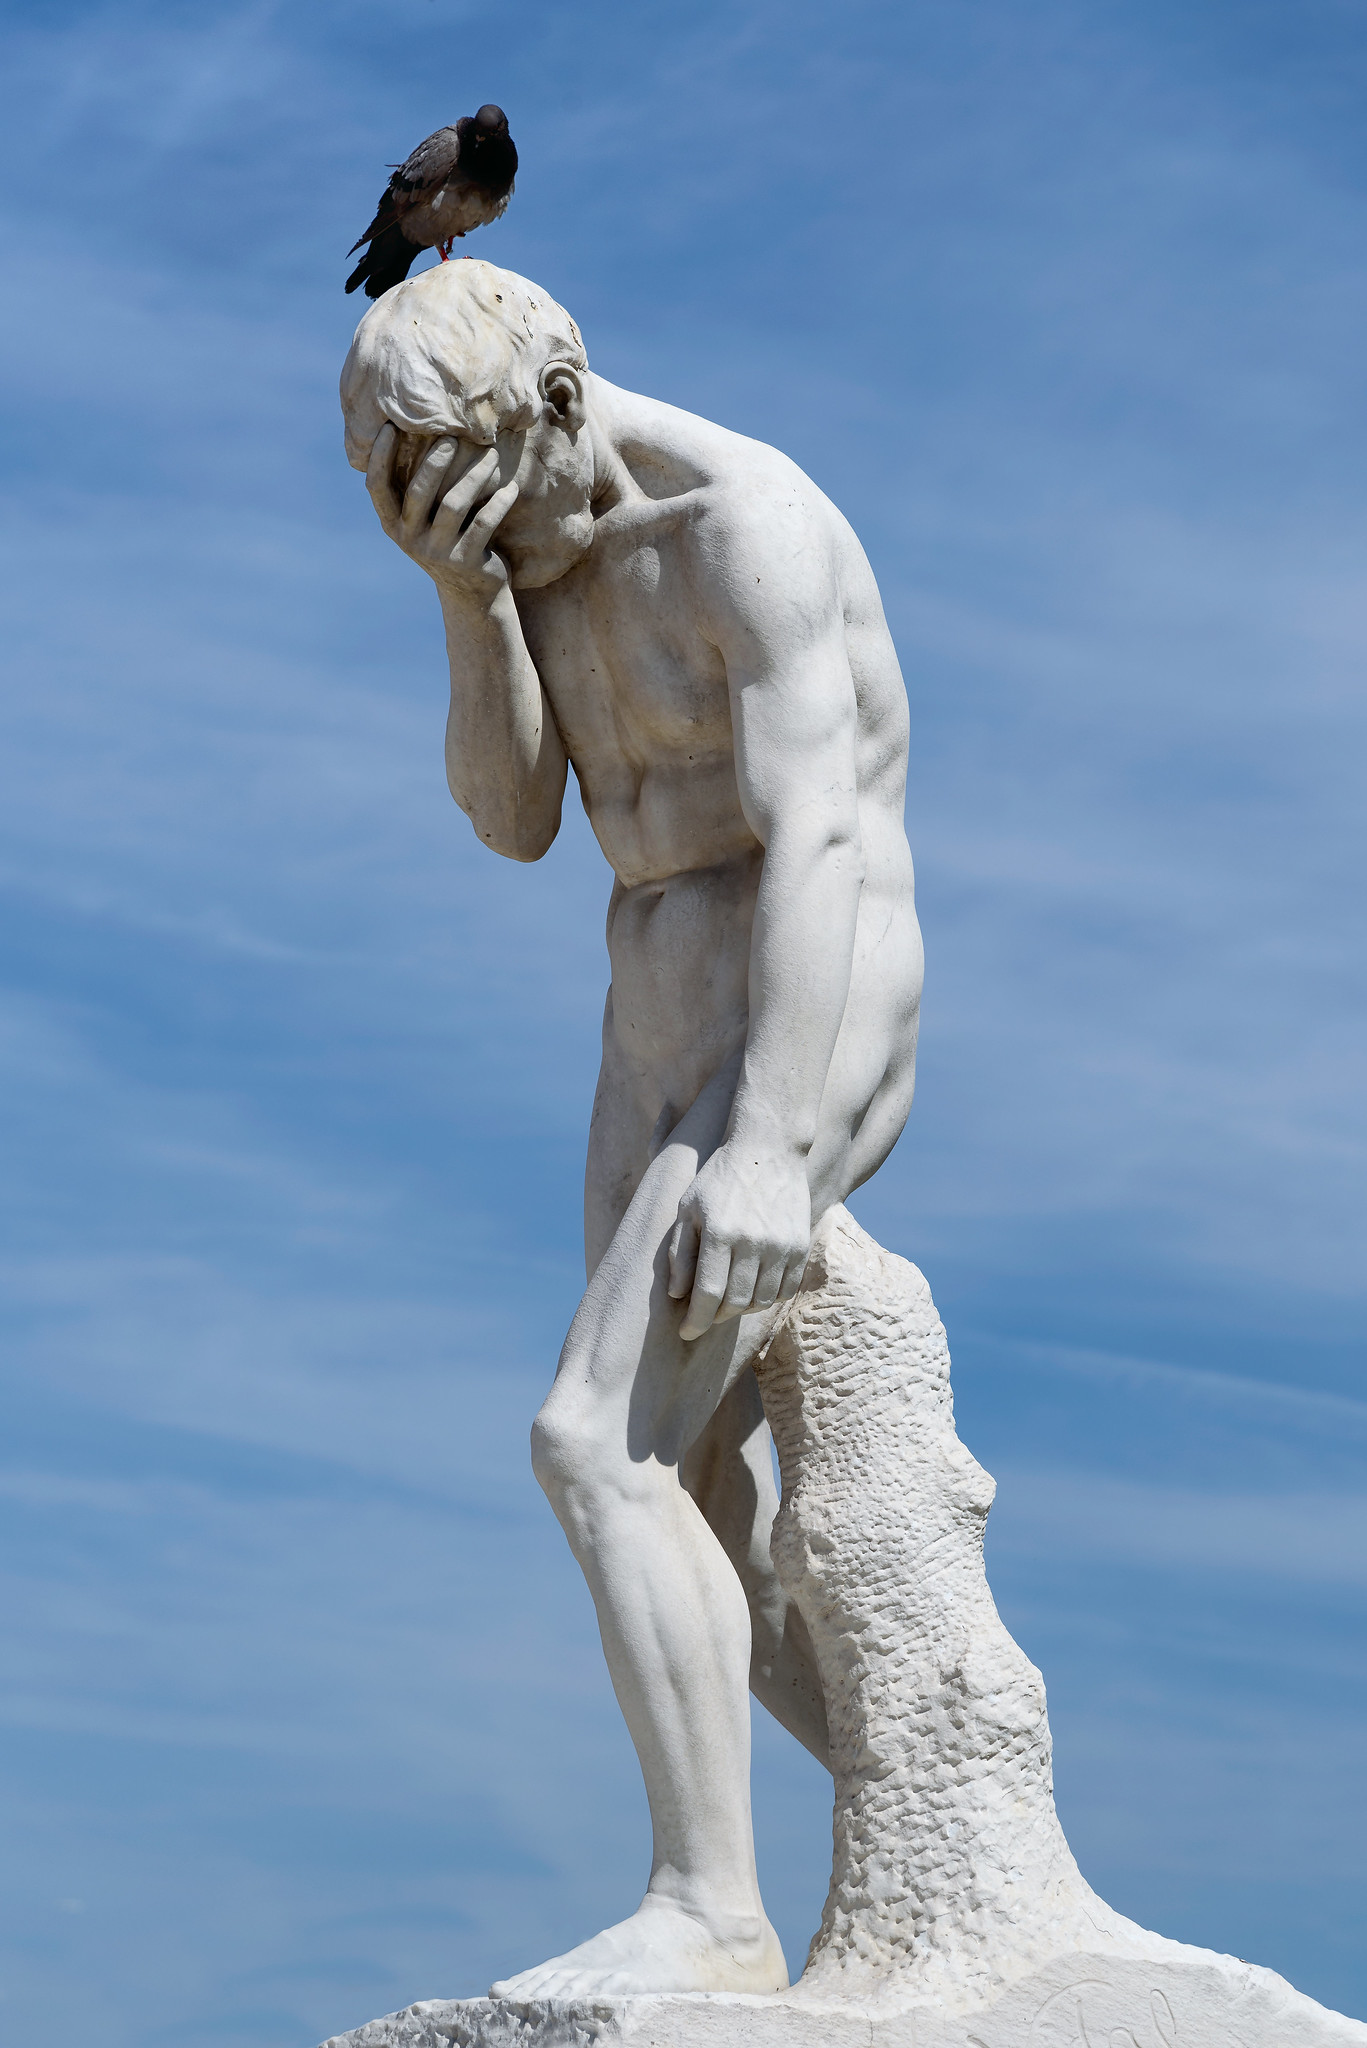
\includegraphics[width=160mm]{facepalm.jpg}
    \end{textblock*}
    \shadowedtitle{140mm - \titlewidth}{25mm}{Why is this hard?}
\end{frame}

% three_files
\begin{frame}[fragile]
    \highlightdef{def}
    \highlightboth{kitchen_import}
    \highlightboth{chef_import}
    \highlightref{ref}
    \frametitle{Multiple files}
    \begin{center}
    \begin{minipage}[t]{22.5em}
    \begin{center}
        
\includegraphics[height=2em]{icons/pan.png}
    \end{center}
    \vskip -1em
    \begin{minipage}[t]{7em}
    \begin{minted}[label=stove.py]{python}
        def bake():
            pass

        def ?\tikzmark{def_start}?broil?\tikzmark{def_end}?():
            pass

        def saute():
            pass
    \end{minted}
    \end{minipage}
    \hspace{0.5em}
    \begin{minipage}[t]{15em}
    \begin{minted}[label=kitchen.py]{python}
        from stove import ?\tikzmark{kitchen_import_start}?*?\tikzmark{kitchen_import_end}?
    \end{minted}
    \end{minipage}
    \end{minipage}
    \hspace{0.5em}
    \begin{minipage}[t]{12em}
    \vskip 8em
    \begin{center}
        
\includegraphics[height=2em]{icons/chef.png}
    \end{center}
    \begin{minted}[label=chef.py]{python}
        from kitchen import ?\tikzmark{chef_import_start}?broil?\tikzmark{chef_import_end}?

        ?\tikzmark{ref_start}?broil?\tikzmark{ref_end}?()
    \end{minted}
    \end{minipage}
    \end{center}
    \curvecodeline%
      [-]%
      {[yshift=10pt] pic cs:ref_end}%
      {+(45:1cm) and +(-155:1cm)}%
      {[yshift=-4pt] pic cs:chef_import_start}%
    \curvecodeline%
      [-]%
      {[xshift=10pt, yshift=10pt] pic cs:chef_import_start}%
      {+(90:5cm) and +(75:2cm)}%
      {[xshift=4pt, yshift=10pt] pic cs:kitchen_import_start}%
    \curvecodeline%
      {[xshift=1pt, yshift=-4pt] pic cs:kitchen_import_start}%
      {+(-105:1cm) and +(75:1cm)}%
      {[xshift=-6pt, yshift=10pt] pic cs:def_end}%
\end{frame}

% three_files_updated
\begin{frame}[fragile]
    \frametitle{Code changes over time}
    \highlightdef{def1}
    \highlightdef{def2}
    \highlightboth{import}
    \highlightref{ref}
    \begin{center}
    \begin{minipage}[t]{22.5em}
    \begin{center}
        
\includegraphics[height=2em]{icons/pan.png}
    \end{center}
    \vskip -1em
    \begin{minipage}[t]{7em}
    \begin{minted}[label=stove.py]{python}
        def bake():
            pass

        def ?\tikzmark{def1_start}?broil?\tikzmark{def1_end}?():
            pass

        def saute():
            pass
    \end{minted}
    \end{minipage}
    \hspace{0.5em}
    \begin{minipage}[t]{15em}
    \begin{minted}[label=kitchen.py]{python}
        from stove import *

        def ?\tikzmark{def2_start}?broil?\tikzmark{def2_end}?():
            print("We're broiling!")
            import stove
            return stove.broil()
    \end{minted}
    \end{minipage}
    \end{minipage}
    \hspace{0.5em}
    \begin{minipage}[t]{12em}
    \vskip 8em
    \begin{center}
        
\includegraphics[height=2em]{icons/chef.png}
    \end{center}
    \begin{minted}[label=chef.py]{python}
        from kitchen import ?\tikzmark{import_start}?broil?\tikzmark{import_end}?

        ?\tikzmark{ref_start}?broil?\tikzmark{ref_end}?()
    \end{minted}
    \end{minipage}
    \end{center}
    \curvecodeline%
      [-]%
      {[yshift=10pt] pic cs:ref_end}%
      {+(45:1cm) and +(-155:1cm)}%
      {[yshift=-4pt] pic cs:import_start}%
    \curvecodeline%
      {[xshift=10pt, yshift=10pt] pic cs:import_start}%
      {+(90:5cm) and +(75:2cm)}%
      {[xshift=-6pt, yshift=10pt] pic cs:def2_end}%
\end{frame}

% python_class
\begin{frame}[fragile]
    \frametitle{Type-dependent name resolution}
    \begin{center}
    \highlightdef{def}
    \highlightref{ref}
    \begin{minipage}[t]{25.5em}
    \begin{center}
        
\includegraphics[height=2em]{icons/pan.png}
    \end{center}
    \vskip -1em
    \begin{minipage}[t]{10em}
    \begin{minted}[label=stove.py]{python}
        class?\tikzmark{class}? Stove?\tikzmark{class_def}?(object):
            def bake(self):
                pass

            def ?\tikzmark{def_start}?broil?\tikzmark{def_end}?(self):
                pass

            def saute(self):
                pass
    \end{minted}
    \end{minipage}
    \hspace{0.5em}
    \begin{minipage}[t]{15em}
    \begin{minted}[label=kitchen.py]{python}
        from stove import ?\tikzmark{kitchen_import}?*
    \end{minted}
    \end{minipage}
    \end{minipage}
    \hspace{-5.5em}
    \begin{minipage}[t]{12em}
    \vskip 6em
    \begin{center}
        
\includegraphics[height=2em]{icons/chef.png}
    \end{center}
    \begin{minted}[label=chef.py]{python}
        from kitchen import ?\tikzmark{chef_import}?Stove

        stove?\tikzmark{instance_def}? = Stove?\tikzmark{class_ref}?()
        stove?\tikzmark{instance_ref}?.?\tikzmark{ref_start}?broil?\tikzmark{ref_end}?()
    \end{minted}
    \end{minipage}
    \end{center}
    \curvecodeline%
      [-]%
      {[xshift=-10pt, yshift=-3pt] pic cs:ref_end}%
      {+(-135:0.2cm) and +(-45:0.2cm)}%
      {[xshift=-10pt, yshift=-3pt] pic cs:instance_ref}%
    \curvecodeline%
      [-]%
      {[xshift=-23pt, yshift=2pt] pic cs:instance_ref}%
      {+(180:0.2cm) and +(180:0.2cm)}%
      {[xshift=-23pt, yshift=2pt] pic cs:instance_def}%
    \curvecodeline%
      [-]%
      {[xshift=-10pt, yshift=8pt] pic cs:instance_def}%
      {+(65:0.3cm) and +(115:0.3cm)}%
      {[xshift=-10pt, yshift=8pt] pic cs:class_ref}%
    \curvecodeline%
      [-]%
      {[xshift=-4pt, yshift=-3pt] pic cs:class_ref}%
      {+(-35:0.5cm) and +(-90:1cm)}%
      {[xshift=10pt, yshift=-3pt] pic cs:chef_import}%
    \curvecodeline%
      [-]%
      {[xshift=10pt, yshift=10pt] pic cs:chef_import}%
      {+(90:3cm) and +(-90:1cm)}%
      {[xshift=2pt, yshift=-3pt] pic cs:kitchen_import}%
    \curvecodeline%
      [-]%
      {[xshift=2pt, yshift=10pt] pic cs:kitchen_import}%
      {+(90:2cm) and +(90:2cm)}%
      {[xshift=-10pt, yshift=8pt] pic cs:class_def}%
    \curvecodeline%
      [-]%
      {[xshift=-6pt, yshift=-2pt] pic cs:class_def}%
      {+(-45:2cm) and +(90:2cm)}%
      {[xshift=4pt, yshift=10pt] pic cs:class_ref}%
    \curvecodeline%
      [-]%
      {[xshift=4pt, yshift=-3pt] pic cs:class_ref}%
      {+(-90:2.5cm) and +(-90:6.5cm)}%
      {[xshift=-10pt, yshift=-2pt] pic cs:class}%
    \curvecodeline%
      {[xshift=-10pt, yshift=8pt] pic cs:class}%
      {+(75:1cm) and +(115:1cm)}%
      {[xshift=-10pt, yshift=6pt] pic cs:def_end}%
\end{frame}


\begin{frame}
    \begin{textblock*}{160mm}(0mm,0mm)
        \only<1>{
            \picturecredit{Mark Gunn}{This just tern'ed into a swarm!}{CC-BY-2.0}{https://flic.kr/p/P11JH1}
            \adjincludegraphics[Trim=0 0 0 1.5in, width=160mm]{terns.jpg}
        }
    \end{textblock*}
    \begin{textblock*}{80mm}(80mm,0mm)
        \only<2>{\adjincludegraphics[Trim=0 0 0 1.5in, width=160mm, Clip={0.5\width} 0 0 0]{terns.jpg}}
    \end{textblock*}

    \begin{onlyenv}<2>
    \frametitle{SCALE}
    200 million repositories and counting
    \vskip 1em
    2 billion contributions \\
    in the last 12 months
    \vskip 1em
    500 programming languages
    \end{onlyenv}
\end{frame}


\begin{frame}
    \begin{textblock*}{160mm}(0mm,-15mm)
        \picturecredit{Katja Schulz}{Inchworm}{CC-BY-2.0}{https://flic.kr/p/PJMP4w}
        \adjincludegraphics[width=160mm]{inchworm.jpg}
    \end{textblock*}
    \shadowedtitle{26mm}{5mm}{Incremental processing}
\end{frame}

\begin{frame}[fragile]
    \begin{textblock*}{160mm}(0mm,-8.5mm)
    \begin{Verbatim}
    7da8cb7380af9a19fb905a263ca247676ccbbd06 ext/requests-logo.ai
    80406e7c06fc0d7c961fdd2bc1c6f8d7f69c1a54 ext/requests-logo.svg
    c1fa878547d8a3fb38689ed0fdad438a0ddb4329 pytest.ini
    9a899df67fb619d871db8b62eea9c1ed436c3a79 requests/__init__.py
    9844f740abea47edbe57cb01d181b341d021ffb1 requests/__version__.py
    759d9a56ba0102bb3b7b3abfcfae6731a2ecc243 requests/_internal_utils.py
    fa4d9b3cc9a2cf6dc2465958387f32193b431410 requests/adapters.py
    88cfdcebbf51d7bfb7b35579085bf985c6926818 requests/api.py
    34e7c8b8fc2daa3229423bc9c6ad6e39c3b3d41a requests/auth.py
    d1a378d787d5a220ef2df694c5cbcd6b4015cbea requests/certs.py
    c44b35efb984650802c40efbc5281b875bae4adc requests/compat.py
    56fccd9c2570d2a31365ed11278fd1b6ecc2aa54 requests/cookies.py
    a80cad80f14411ddf0ba86070d1a65c78dbf7878 requests/exceptions.py
    e53d35ef6dec122aa4aba941b9c555997a35d143 requests/help.py
    7a51f212c8a08fc6a04e509e89d8dcc85185df77 requests/hooks.py
    62dcd0b7c8c64399ad0d317fcfa926e40388d968 requests/models.py
    7232fe0ff7e85083d47d624532f29badd7c854d0 requests/packages.py
    d73d700fa6baa975ab9b10fbdb186bccdb9d3610 requests/sessions.py
    813e8c4e62fdcbbfcb73e2f52e187e0c3c5b84d7 requests/status_codes.py
    da930e2852049feb2b6e262d442b9cc25ecb2d94 requests/structures.py
    8170a8d2c45dc6d9dbb44abc4d5ce4d7c548463d requests/utils.py
    ed8a958e0a8da154b0db9b1edca6e47e5dae146a setup.cfg
    3dce2965e210359f4c96f174b860e6f403d09ad9 setup.py
    \end{Verbatim}
    \end{textblock*}
\end{frame}

\begin{frame}[fragile]
    \begin{textblock*}{160mm}(0mm,-8.5mm)
    \begin{Verbatim}[formatcom=\color{grayish},commandchars=\\\{\}]
    7da8cb7380af9a19fb905a263ca247676ccbbd06 ext/requests-logo.ai
    80406e7c06fc0d7c961fdd2bc1c6f8d7f69c1a54 ext/requests-logo.svg
    c1fa878547d8a3fb38689ed0fdad438a0ddb4329 pytest.ini
    9a899df67fb619d871db8b62eea9c1ed436c3a79 requests/__init__.py
    9844f740abea47edbe57cb01d181b341d021ffb1 requests/__version__.py
    759d9a56ba0102bb3b7b3abfcfae6731a2ecc243 requests/_internal_utils.py
    fa4d9b3cc9a2cf6dc2465958387f32193b431410 requests/adapters.py
    88cfdcebbf51d7bfb7b35579085bf985c6926818 requests/api.py
    \textcolor{black}{eeface39ae62c3975ff535e6b1f79f2c28fbf888 requests/auth.py}
    d1a378d787d5a220ef2df694c5cbcd6b4015cbea requests/certs.py
    c44b35efb984650802c40efbc5281b875bae4adc requests/compat.py
    56fccd9c2570d2a31365ed11278fd1b6ecc2aa54 requests/cookies.py
    a80cad80f14411ddf0ba86070d1a65c78dbf7878 requests/exceptions.py
    e53d35ef6dec122aa4aba941b9c555997a35d143 requests/help.py
    7a51f212c8a08fc6a04e509e89d8dcc85185df77 requests/hooks.py
    \textcolor{black}{457b8412d7cabde41125aaf5ed81fbc86e53eacf requests/models.py}
    7232fe0ff7e85083d47d624532f29badd7c854d0 requests/packages.py
    \textcolor{black}{759ecbe03cd52eb7b3ab966c91ad7921a52620eb requests/sessions.py}
    813e8c4e62fdcbbfcb73e2f52e187e0c3c5b84d7 requests/status_codes.py
    da930e2852049feb2b6e262d442b9cc25ecb2d94 requests/structures.py
    \textcolor{black}{28c9366e2f78bc627c5fee05bddc3697c11bcfc7 requests/utils.py}
    ed8a958e0a8da154b0db9b1edca6e47e5dae146a setup.cfg
    3dce2965e210359f4c96f174b860e6f403d09ad9 setup.py
    \end{Verbatim}
    \end{textblock*}
\end{frame}


\begin{frame}[fragile]
    \begin{center}
    \scalebox{0.6}{
    \begin{tikzpicture}
        \node (root)       [highlight node on={<17,24>}]
                           [root node]                            {};

        \node (stove)      [highlight node on={<25>}]
                           [definition]  [below=4em of root] {\PopSymbol{stove}};
        \node (dot)        [highlight node on={<26>}]
                           [pop]         [left=of stove]          {\PopSymbol{.}};
        \node (s1)         [highlight node on={<27>}]
                           [anon scope]  [left=of dot]            {};

        \node (s2)         [highlight node on={<28>}]
                           [anon scope]  [above=\scopegap of s1]  {};
        \node (Stove def)  [highlight node on={<29>}]
                           [definition]  [left=of s2]             {\PopSymbol{Stove}};
        \node (s3)         [anon scope]  [above=\scopegap of s2]  {};

        \node (call)       [highlight node on={<30>}]
                           [pop]  [left=of Stove def]             {\PopSymbol{()}};
        \node (instance)   [highlight node on={<31>}]
                           [exported scope]  [left=of call]       {IM};
        \node (member)     [highlight node on={<32>}]
                           [pop]  [left=of instance]              {\PopSymbol{.}};
        \node (m1)         [highlight node on={<33>}]
                           [anon scope]  [above=of member]         {};

        \setwidestsymbol{\PopSymbol{broil}}
        \node (m2)         [highlight node on={<34>}]
                           [anon scope]  [above=\scopegap of m1]  {};
        \node (saute def)  [definition]  [left=of m2]             {\sized{\PopSymbol{saute}}};
        \node (m3)         [highlight node on={<35>}]
                           [anon scope]  [above=\scopegap of m2]  {};
        \node (broil def)  [highlight node on={<2,36>}]
                           [definition]  [left=of m3]             {\sized{\PopSymbol{broil}}};
        \node (m4)         [anon scope]  [above=\scopegap of m3]  {};
        \node (bake def)   [definition]  [left=of m4]             {\sized{\PopSymbol{bake}}};
        \node (m5)         [anon scope]  [above=\scopegap of m4]  {};

        \path [-Stealth]
          (root)      edge [highlight inner edge on=<2>, show path on=<25>] (stove)
          (stove)     edge [highlight inner edge on=<2>, show path on=<26>] (dot)
          (dot)       edge [highlight inner edge on=<2>, show path on=<27>] (s1)
          (s1)        edge [highlight inner edge on=<2>, show path on=<28>] (s2)
          (s2)        edge (s3)
                      edge [highlight inner edge on=<2>, show path on=<29>] (Stove def)
          (Stove def) edge [highlight inner edge on=<2>, show path on=<30>] (call)
          (call)      edge [highlight inner edge on=<2>, show path on=<31>] (instance)
          (instance)  edge [highlight inner edge on=<2>, show path on=<32>] (member)
          (member)    edge [highlight inner edge on=<2>, show path on=<33>] (m1)
          (m1)        edge [highlight inner edge on=<2>, show path on=<34>] (m2)
          (m2)        edge [highlight inner edge on=<2>, show path on=<35>] (m3)
                      edge (saute def)
          (m3)        edge (m4)
                      edge [highlight end edge on=<2>, show path on=<36>]   (broil def)
          (m4)        edge (m5)
                      edge (bake def)
          ;

        \node (kitchen)      [highlight node on={<18>}]
                             [definition]  [above=4em of root]  {\PopSymbol{kitchen}};
        \node (dot)          [highlight node on={<19>}]
                             [pop]         [left=of kitchen]        {\PopSymbol{.}};
        \node (k1)           [highlight node on={<20>}]
                             [anon scope]  [left=of dot]            {};

        \node (k2)           [highlight node on={<21>}]
                             [anon scope]  [above=\scopegap of k1]  {};
        \node (reimport dot) [highlight node on={<22>}]
                             [push]        [left=of k2]             {\PushSymbol{.}};
        \node (reimport mod) [highlight node on={<23>}]
                             [push]        [left=of reimport dot]   {\PushSymbol{stove}};
        \node (k3)           [anon scope]  [above=\scopegap of k2]  {};

        \path [-Stealth]
          (root)         edge [highlight inner edge on=<2>, show path on=<18>] (kitchen)
          (kitchen)      edge [highlight inner edge on=<2>, show path on=<19>] (dot)
          (dot)          edge [highlight inner edge on=<2>, show path on=<20>] (k1)
          (k1)           edge [highlight inner edge on=<2>, show path on=<21>] (k2)
          (k2)           edge (k3)
                         edge [highlight inner edge on=<2>, show path on=<22>] (reimport dot)
          (reimport dot) edge [highlight inner edge on=<2>, show path on=<23>] (reimport mod)
          (reimport mod) edge [overlay, in control=+(135:2cm), out control=+(-90:1.5cm)]
                              [highlight inner edge on=<2>, show path on=<24>] (root)
          ;

        \node (chef)       [definition]  [right=3em of root]      {\PopSymbol{chef}};
        \node (dot)        [pop]         [right=of chef]          {\PopSymbol{.}};
        \node (c1)         [anon scope]  [above=of dot]           {};

        \node (c2)         [highlight node on={<7>}]
                           [anon scope]  [above=\scopegap of c1]  {};
        \node (stove ref)  [highlight node on={<6>}]
                           [reference]   [right=of c2]            {\PushSymbol{stove}};
        \node (member dot) [highlight node on={<5>}]
                           [push]        [right=of stove ref]     {\PushSymbol{.}};
        \node (broil ref)  [highlight node on={<2,4>}]
                           [reference]   [right=of member dot]    {\PushSymbol{broil}};
        \node (c3)         [highlight node on={<8>}]
                           [anon scope]  [above=\scopegap of c2]  {};
        \node (stove def)  [highlight node on={<9>}]
                           [definition]  [right=of c3]            {\PopSymbol{stove}};
        \node (Stove call) [highlight node on={<10>}]
                           [push]        [right=of stove def]     {\PushSymbol{()}};
        \node (Stove ref)  [highlight node on={<11>}]
                           [reference]   [right=of Stove call]    {\PushSymbol{Stove}};
        \node (c4)         [highlight node on={<12>}]
                           [anon scope]  [above=\scopegap of c3]  {};
        \node (import def) [highlight node on={<13>}]
                           [pop]         [right=of c4]            {\PopSymbol{Stove}};
        \node (import ref) [highlight node on={<14>}]
                           [push]        [right=of import def]    {\PushSymbol{Stove}};
        \node (import dot) [highlight node on={<15>}]
                           [push]        [right=of import ref]    {\PushSymbol{.}};
        \node (import mod) [highlight node on={<16>}]
                           [push]        [right=of import dot]    {\PushSymbol{kitchen}};
        \node (c5)         [anon scope]  [above=\scopegap of c4]  {};

        \path [-Stealth]
          (root)       edge (chef)
          (chef)       edge (dot)
          (dot)        edge (c1)
          (c1)         edge (c2)
          (broil ref)  edge [highlight inner edge on=<2>, show path on=<5>] (member dot)
          (member dot)  edge [highlight inner edge on=<2>, show path on=<6>] (stove ref)
          (stove ref)  edge [highlight inner edge on=<2>, show path on=<7>] (c2)
          (c2)         edge [highlight inner edge on=<2>, show path on=<8>] (c3)
          (c3)         edge (c4)
                       edge [highlight inner edge on=<2>, show path on=<9>] (stove def)
          (stove def)  edge [highlight inner edge on=<2>, show path on=<10>] (Stove call)
          (Stove call) edge [highlight inner edge on=<2>, show path on=<11>] (Stove ref)
          (Stove ref)  edge [highlight inner edge on=<2>, show path on=<12>] 
                            [in control=+(-65:1cm), out control=+(90:1cm)] (c4)
          (c4)         edge (c5)
                       edge [highlight inner edge on=<2>, show path on=<13>] (import def)
          (import def) edge [highlight inner edge on=<2>, show path on=<14>] (import ref)
          (import ref) edge [highlight inner edge on=<2>, show path on=<15>] (import dot)
          (import dot) edge [highlight inner edge on=<2>, show path on=<16>] (import mod)
          (import mod) edge [overlay, in control=+(-45:3cm), out control=+(-90:6cm)]
                            [highlight inner edge on=<2>, show path on=<17>] (root)
          ;
    \end{tikzpicture}
    }
    \vskip 2em
    \begin{tabular}{m{5em} m{14em}}
        \only<3- >                   {\textsmaller[2]{Symbol stack:}} &
        \only<3,36>                  {$\nilsymbolstack$}
        \only<4,32-35>               {$\symbolstack{broil}$}
        \only<5,9,30-31>             {$\symbolstack{.broil}$}
        \only<6-8>                   {$\symbolstack{stove.broil}$}
        \only<10,13,29>              {$\symbolstack{().broil}$}
        \only<11-12,14,19-21,26-28>  {$\symbolstack{Stove().broil}$}
        \only<15,18,22,25>           {$\symbolstack{.Stove().broil}$}
        \only<16-17>                 {$\symbolstack{kitchen.Stove().broil}$}
        \only<23-24>                 {$\symbolstack{stove.Stove().broil}$}
    \end{tabular}
    \end{center}
\end{frame}


\section{Partial paths}

\begin{frame}
    \begin{textblock*}{160mm}(0mm,0mm)
        \picturecredit{Seattle Municipal Archives}{West Seattle Bridge under construction, circa 1983}{CC-BY-2.0}{https://flic.kr/p/7jKWYi}
        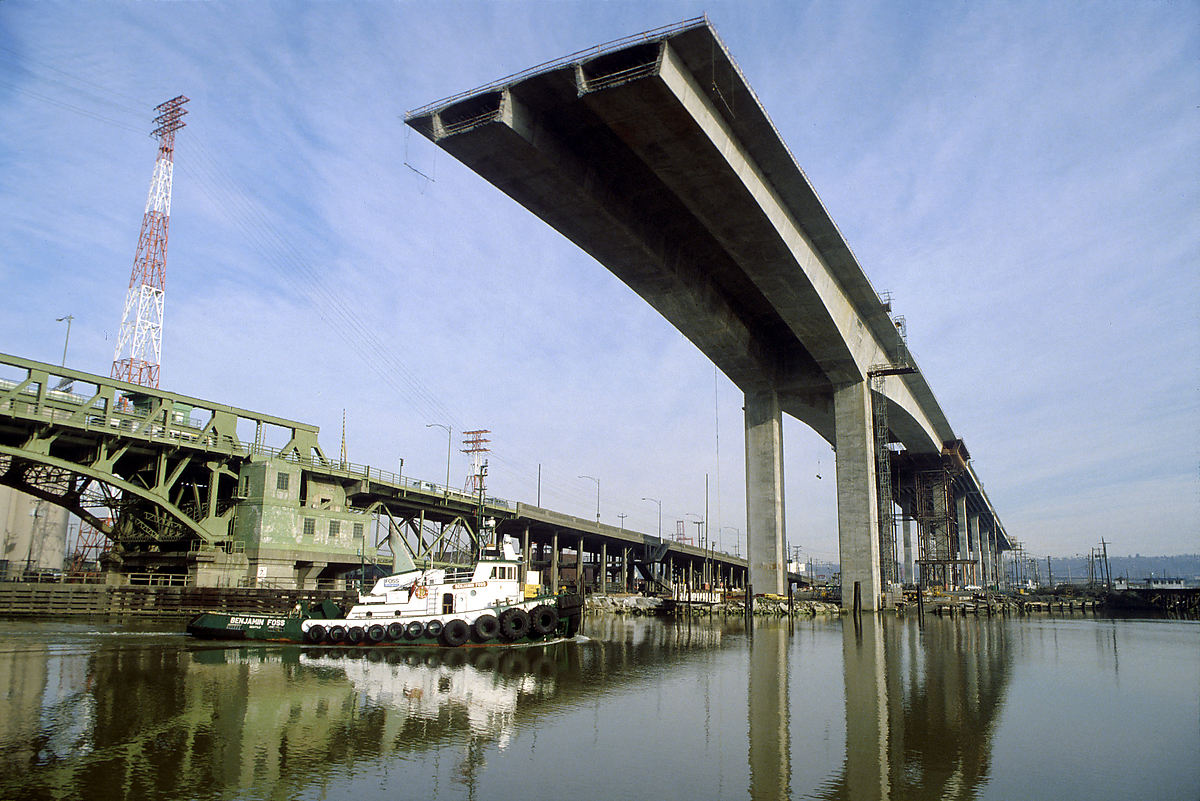
\includegraphics[width=160mm]{bridge.jpg}
    \end{textblock*}
    \shadowedtitle{150mm - \titlewidth}{10mm}{Partial paths}
\end{frame}

\begin{frame}[t,fragile]
    \frametitle{Per-file stack graphs}

    \begin{center}

    \begin{minipage}{10em}
    \begin{minted}[label={\tikzmark{file_start}stove.py\tikzmark{file_end}}]{python}
        ?\tikzmark{class_start}?class?\tikzmark{class_end}? ?\tikzmark{Stove_start}?Stove?\tikzmark{Stove_end}?(object):
            def bake(self):
                pass

            def ?\tikzmark{def_start}?broil?\tikzmark{def_end}?(self):
                pass

            def saute(self):
                pass
    \end{minted}
    \end{minipage}
    \hspace{2em}
    \scalebox{0.6}{
    \begin{tikzpicture}[baseline={(current bounding box.center)}]
        \node (root)       [root node]                            {};
        \node (stove)      [definition]  [below=4em of root] {stove};
        \node (dot)        [pop]         [left=of stove]          {.};
        \node (s1)         [anon scope]  [left=of dot]            {};

        \node (s2)         [anon scope]  [above=\scopegap of s1]  {};
        \node (Stove def)  [definition]  [left=of s2]             {Stove};
        \node (s3)         [anon scope]  [above=\scopegap of s2]  {};

        \node (call)       [pop]  [left=of Stove def]             {()};
        \node (instance)   [exported scope]  [left=of call]       {IM};
        \node (member)     [pop]  [left=of instance]              {.};
        \node (m1)         [anon scope]  [left=of member]         {};

        \setwidestsymbol{broil}
        \node (m2)         [anon scope]  [above=\scopegap of m1]  {};
        \node (saute def)  [definition]  [left=of m2]             {\sized{saute}};
        \node (m3)         [anon scope]  [above=\scopegap of m2]  {};
        \node (broil def)  [definition]  [left=of m3]             {\sized{broil}};
        \node (m4)         [anon scope]  [above=\scopegap of m3]  {};
        \node (bake def)   [definition]  [left=of m4]             {\sized{bake}};
        \node (m5)         [anon scope]  [above=\scopegap of m4]  {};

        \path [-Stealth]
          (root)      edge [highlight inner edge on=<2- >] (stove)
          (stove)     edge [highlight inner edge on=<2- >] (dot)
          (dot)       edge [highlight inner edge on=<2- >] (s1)
          (s1)        edge [highlight inner edge on=<2- >] (s2)
          (s2)        edge (s3)
                      edge [highlight inner edge on=<2- >] (Stove def)
          (Stove def) edge [highlight inner edge on=<2- >] (call)
          (call)      edge [highlight end edge on=<2- >] (instance)
          (instance)  edge (member)
          (member)    edge (m1)
          (m1)        edge (m2)
          (m2)        edge (m3)
                      edge (saute def)
          (m3)        edge (m4)
                      edge (broil def)
          (m4)        edge (m5)
                      edge (bake def)
          ;
    \end{tikzpicture}
    }
    \hspace{3em}

    \vskip 2em
    \uncover<3- >{\partialpath
        {\symbolstack{stove.Stove()} \cdot \psi}
        {\node [root node]{}}
        {\node [exported scope] {IM}}
        {\psi}}
    \vskip 0.75em
    \uncover<4>{
        Invoking \texttt{stove.Stove} \\
        gives you an instance of the \texttt{Stove} class. \\
    }

    \end{center}
\end{frame}


\begin{frame}[t,fragile]
    \frametitle{Per-file stack graphs}

    \begin{center}

    \begin{minipage}{10em}
    \begin{minted}[label={\tikzmark{file_start}stove.py\tikzmark{file_end}}]{python}
        ?\tikzmark{class_start}?class?\tikzmark{class_end}? ?\tikzmark{Stove_start}?Stove?\tikzmark{Stove_end}?(object):
            def bake(self):
                pass

            def ?\tikzmark{def_start}?broil?\tikzmark{def_end}?(self):
                pass

            def saute(self):
                pass
    \end{minted}
    \end{minipage}
    \hspace{2em}
    \scalebox{0.6}{
    \begin{tikzpicture}[baseline={(current bounding box.center)}]
        \node (root)       [root node]                            {};
        \node (stove)      [definition]  [below=4em of root] {stove};
        \node (dot)        [pop]         [left=of stove]          {.};
        \node (s1)         [anon scope]  [left=of dot]            {};

        \node (s2)         [anon scope]  [above=\scopegap of s1]  {};
        \node (Stove def)  [definition]  [left=of s2]             {Stove};
        \node (s3)         [anon scope]  [above=\scopegap of s2]  {};

        \node (call)       [pop]  [left=of Stove def]             {()};
        \node (instance)   [exported scope]  [left=of call]       {IM};
        \node (member)     [pop]  [left=of instance]              {.};
        \node (m1)         [anon scope]  [left=of member]         {};

        \setwidestsymbol{broil}
        \node (m2)         [anon scope]  [above=\scopegap of m1]  {};
        \node (saute def)  [definition]  [left=of m2]             {\sized{saute}};
        \node (m3)         [anon scope]  [above=\scopegap of m2]  {};
        \node (broil def)  [definition]  [left=of m3]             {\sized{broil}};
        \node (m4)         [anon scope]  [above=\scopegap of m3]  {};
        \node (bake def)   [definition]  [left=of m4]             {\sized{bake}};
        \node (m5)         [anon scope]  [above=\scopegap of m4]  {};

        \path [-Stealth]
          (root)      edge (stove)
          (stove)     edge (dot)
          (dot)       edge (s1)
          (s1)        edge (s2)
          (s2)        edge (s3)
                      edge (Stove def)
          (Stove def) edge (call)
          (call)      edge (instance)
          (instance)  edge [highlight inner edge on=<1- >] (member)
          (member)    edge [highlight inner edge on=<1- >] (m1)
          (m1)        edge [highlight inner edge on=<1- >] (m2)
          (m2)        edge [highlight inner edge on=<1- >] (m3)
                      edge (saute def)
          (m3)        edge (m4)
                      edge [highlight end edge on=<1- >] (broil def)
          (m4)        edge (m5)
                      edge (bake def)
          ;
    \end{tikzpicture}
    }
    \hspace{3em}

    \vskip 2em
    \uncover<2- >{\partialpath
        {\symbolstack{.broil} \cdot \psi}
        {\node [exported scope] {IM}}
        {\node [definition]{\PopSymbol{broil}}}
        {\psi}}
    \vskip 0.75em
    \uncover<3>{
        The \texttt{Stove} class \\
        has an instance member named \texttt{broil} \\
        defined at \textsl{stove.py:5:9}. \\
    }

    \end{center}
\end{frame}


\begin{frame}[fragile]
    \frametitle{Per-file stack graphs}

    \begin{center}

    \begin{minipage}[t]{15em}
    \begin{minted}[label={\tikzmark{file_start}kitchen.py\tikzmark{file_end}}]{python}
        from ?\tikzmark{import_start}?stove?\tikzmark{import_end}? import ?\tikzmark{star_start}?*?\tikzmark{star_end}?
    \end{minted}
    \end{minipage}
    \hspace{2em}
    \scalebox{0.6}{
        \begin{tikzpicture}[baseline={([yshift=1em] current bounding box.center)}]
        \node (root)         [root node]                            {};
        \node (kitchen)      [definition]  [above=4em of root]  {kitchen};
        \node (dot)          [pop]         [left=of kitchen]        {.};
        \node (k1)           [anon scope]  [left=of dot]            {};

        \node (k2)           [anon scope]  [above=\scopegap of k1]  {};
        \node (reimport dot) [push]        [left=of k2]             {.};
        \node (reimport mod) [push]        [left=of reimport dot]   {stove};
        \node (k3)           [anon scope]  [above=\scopegap of k2]  {};

        \path [-Stealth]
          (root)         edge [highlight inner edge on=<2- >] (kitchen)
          (kitchen)      edge [highlight inner edge on=<2- >] (dot)
          (dot)          edge [highlight inner edge on=<2- >] (k1)
          (k1)           edge [highlight inner edge on=<2- >] (k2)
          (k2)           edge (k3)
                         edge [highlight inner edge on=<2- >] (reimport dot)
          (reimport dot) edge [highlight inner edge on=<2- >] (reimport mod)
          (reimport mod) edge [overlay, in control=+(135:2cm), out control=+(-90:1.5cm)]
                              [highlight end edge on=<2- >] (root)
          ;
    \end{tikzpicture}
    }

    \vskip 3em
    \uncover<3- >{\partialpath
        {\symbolstack{kitchen.} \cdot \psi}
        {\node [root node] {}}
        {\node [root node] {}}
        {\symbolstack{stove.} \cdot \psi}}
    \vskip 0.75em
    \uncover<4>{
        If you are looking for \texttt{kitchen.[anything]} \\
        then you might find it at \texttt{stove.[anything]}. \\
    }

    \end{center}
\end{frame}


\begin{frame}[fragile]
    \frametitle{Per-file stack graphs}

    \begin{center}

    \begin{minipage}{12em}
    \begin{minted}[label=chef.py]{python}
        from kitchen import ?\tikzmark{chef_import}?Stove

        stove?\tikzmark{instance_def}? = Stove?\tikzmark{class_ref}?()
        stove?\tikzmark{instance_ref}?.?\tikzmark{ref_start}?broil?\tikzmark{ref_end}?()
    \end{minted}
    \end{minipage}
    \hspace{-5em}
    \scalebox{0.6}{
        \begin{tikzpicture}[baseline={([yshift=1em] current bounding box.center)}]
        \node (root)       [root node]                            {};
        \node (chef)       [definition]  [right=3em of root]      {chef};
        \node (dot)        [pop]         [right=of chef]          {.};
        \node (c1)         [anon scope]  [right=of dot]           {};

        \node (c2)         [anon scope]  [above=\scopegap of c1]  {};
        \node (stove ref)  [reference]   [right=of c2]            {stove};
        \node (member dot) [push]        [right=of stove ref]     {.};
        \node (broil ref)  [reference]   [right=of member dot]    {broil};
        \node (c3)         [anon scope]  [above=\scopegap of c2]  {};
        \node (stove def)  [definition]  [right=of c3]            {stove};
        \node (Stove call) [push]        [right=of stove def]     {()};
        \node (Stove ref)  [reference]   [right=of Stove call]    {Stove};
        \node (c4)         [anon scope]  [above=\scopegap of c3]  {};
        \node (import def) [pop]         [right=of c4]            {Stove};
        \node (import ref) [push]        [right=of import def]    {Stove};
        \node (import dot) [push]        [right=of import ref]    {.};
        \node (import mod) [push]        [right=of import dot]    {kitchen};
        \node (c5)         [anon scope]  [above=\scopegap of c4]  {};

        \path [-Stealth]
          (root)       edge (chef)
          (chef)       edge (dot)
          (dot)        edge (c1)
          (c1)         edge (c2)
          (broil ref)  edge [highlight inner edge on=<2- >] (member dot)
          (member dot)  edge [highlight inner edge on=<2- >] (stove ref)
          (stove ref)  edge [highlight inner edge on=<2- >] (c2)
          (c2)         edge [highlight inner edge on=<2- >] (c3)
          (c3)         edge (c4)
                       edge [highlight inner edge on=<2- >] (stove def)
          (stove def)  edge [highlight inner edge on=<2- >] (Stove call)
          (Stove call) edge [highlight inner edge on=<2- >] (Stove ref)
          (Stove ref)  edge [highlight inner edge on=<2- >] 
                            [in control=+(-65:1cm), out control=+(90:1cm)] (c4)
          (c4)         edge (c5)
                       edge [highlight inner edge on=<2- >] (import def)
          (import def) edge [highlight inner edge on=<2- >] (import ref)
          (import ref) edge [highlight inner edge on=<2- >] (import dot)
          (import dot) edge [highlight inner edge on=<2- >] (import mod)
          (import mod) edge [overlay, in control=+(-45:3cm), out control=+(-90:6cm)]
                            [highlight end edge on=<2- >] (root)
          ;
    \end{tikzpicture}
    }

    \vskip 3em
    \uncover<3- >{\partialpath
        {\nilsymbolstack}
        {\node [reference] {\PushSymbol{broil}}}
        {\node [root node]{}}
        {\symbolstack{kitchen.Stove().broil}}}
    \vskip 0.75em
    \uncover<4>{
        If you can find what \texttt{kitchen.Stove} resolves to and can call it \\
        then the result should have a member named \texttt{broil} \\
        which the reference at \textsl{chef.py:4:7} resolves to. \\
    }

    \end{center}
\end{frame}


\begin{frame}[fragile]
    \frametitle{Concatenating partial paths}

    \vskip 2em
    \begin{center}
        \begin{minipage}[t]{0.46\textwidth}
            \begin{center}
            \scalebox{0.75}{\partialpath
                {\nilsymbolstack}
                {\node [reference] {\PushSymbol{broil}}}
                {\node [root node]{}}
                {\symbolstack{kitchen.Stove().broil}}}
            \end{center}
        \end{minipage}
        \begin{uncoverenv}<2- >
            \; $+$ \;
        \begin{minipage}[t]{0.46\textwidth}
            \begin{center}
            \scalebox{0.75}{\partialpath
                {\symbolstack{kitchen.} \cdot \psi}
                {\node [root node] {}}
                {\node [root node]{}}
                {\symbolstack{stove.} \cdot \psi}}
            \end{center}
        \end{minipage}
        \end{uncoverenv}
        \vskip 0.5em
        \begin{minipage}[t][1cm][t]{0.46\textwidth}
        \begin{center}
            \scalebox{0.7}{
                \onslide<3>{$\psi = \symbolstack{Stove().broil}$}
            }
        \end{center}
        \end{minipage}
        \vskip 0.5em
        \begin{minipage}[c][2cm][c]{0.46\textwidth}
            \begin{center}
            \smaller[1]
            If you can find what \texttt{kitchen.Stove} \\
            resolves to and can call it, then the \\
            result should have a member \\
            named \texttt{broil} which the reference at \\
            \textsl{chef.py:4:7} resolves to.
            \end{center}
        \end{minipage}
        \begin{uncoverenv}<2- >
            \; $+$ \;
        \begin{minipage}[c][2cm][c]{0.46\textwidth}
            \begin{center}
            \smaller[1]
            If you are looking for \\
            \texttt{kitchen.[anything]} \\
            then you might find it at \\
            \texttt{stove.[anything]}. \\
            \end{center}
        \end{minipage}
        \end{uncoverenv}
    \end{center}
\end{frame}


\begin{frame}[fragile]
    \frametitle{Concatenating partial paths}

    \vskip 2em
    \begin{center}
        \begin{minipage}[t]{0.46\textwidth}
            \begin{center}
            \scalebox{0.75}{\partialpath
                {\nilsymbolstack}
                {\node [reference] {\PushSymbol{broil}}}
                {\node [root node]{}}
                {\symbolstack{stove.Stove().broil}}}
            \end{center}
        \end{minipage}
        \begin{uncoverenv}<2- >
            \; $+$ \;
        \begin{minipage}[t]{0.46\textwidth}
            \begin{center}
            \scalebox{0.75}{\partialpath
                {\symbolstack{stove.Stove()} \cdot \psi}
                {\node [root node]{}}
                {\node [exported scope] {IM}}
                {\psi}}
            \end{center}
        \end{minipage}
        \end{uncoverenv}
        \vskip 0.5em
        \begin{minipage}[t][1cm][t]{0.46\textwidth}
        \begin{center}
            \scalebox{0.7}{
                \onslide<3>{$\psi = \symbolstack{.broil}$}
            }
        \end{center}
        \end{minipage}
        \vskip 0.5em
        \begin{minipage}[c][2cm][c]{0.46\textwidth}
            \begin{center}
            \smaller[1]
            If you can find what \texttt{stove.Stove} \\
            resolves to and can call it, then the \\
            result should have a member \\
            named \texttt{broil} which the reference at \\
            \textsl{chef.py:4:7} resolves to.
            \end{center}
        \end{minipage}
        \begin{uncoverenv}<2- >
            \; $+$ \;
        \begin{minipage}[c][2cm][c]{0.46\textwidth}
            \begin{center}
            \smaller[1]
            Invoking \texttt{stove.Stove} gives you \\
            an instance of the \texttt{Stove} class.
            \end{center}
        \end{minipage}
        \end{uncoverenv}
    \end{center}
\end{frame}


\begin{frame}[fragile]
    \frametitle{Concatenating partial paths}

    \vskip 2em
    \begin{center}
        \begin{minipage}[t]{0.46\textwidth}
            \begin{center}
            \scalebox{0.75}{\partialpath
                {\nilsymbolstack}
                {\node [reference] {\PushSymbol{broil}}}
                {\node [exported scope]{IM}}
                {\symbolstack{.broil}}}
            \end{center}
        \end{minipage}
        \begin{uncoverenv}<2- >
            \; $+$ \;
        \begin{minipage}[t]{0.46\textwidth}
            \begin{center}
            \scalebox{0.75}{\partialpath
                {\symbolstack{.broil} \cdot \psi}
                {\node [exported scope] {IM}}
                {\node [definition]{\PopSymbol{broil}}}
                {\psi}}
            \end{center}
        \end{minipage}
        \end{uncoverenv}
        \vskip 0.5em
        \begin{minipage}[t][1cm][t]{0.46\textwidth}
        \begin{center}
            \scalebox{0.7}{
                \onslide<3>{$\psi = \nilsymbolstack$}
            }
        \end{center}
        \end{minipage}
        \vskip 0.5em
        \begin{minipage}[c][2cm][c]{0.46\textwidth}
            \begin{center}
            \smaller[1]
            The \texttt{Stove} class \\
            should have a member \\
            named \texttt{broil} which the reference at \\
            \textsl{chef.py:4:7} resolves to.
            \end{center}
        \end{minipage}
        \begin{uncoverenv}<2- >
            \; $+$ \;
        \begin{minipage}[c][2cm][c]{0.46\textwidth}
            \begin{center}
            \smaller[1]
            The \texttt{Stove} class has an \\
            instance member named \texttt{broil} \\
            defined at \textsl{stove.py:5:9}.
            \end{center}
        \end{minipage}
        \end{uncoverenv}
    \end{center}
\end{frame}


\begin{frame}[fragile]
    \frametitle{Concatenating partial paths}

    \vskip 2em
    \begin{center}
        \begin{minipage}[t]{0.46\textwidth}
            \begin{center}
            \scalebox{0.75}{\partialpath
                {\nilsymbolstack}
                {\node [reference] {\PushSymbol{broil}}}
                {\node [definition]{\PopSymbol{broil}}}
                {\nilsymbolstack}}
            \end{center}
        \end{minipage}
        \phantom{\; $+$ \;}
        \begin{minipage}[t]{0.46\textwidth}
            \strut
        \end{minipage}
        \vskip 0.5em
        \begin{minipage}[t][1cm][t]{0.46\textwidth}
        \begin{center}
            \scalebox{0.7}{
                \vphantom{$\psi = \symbolstack{.broil}$}
            }
        \end{center}
        \end{minipage}
        \vskip 0.5em
        \begin{minipage}[c][2cm][c]{0.46\textwidth}
            \begin{center}
            \smaller[1]
            The definition at \textsl{stove.py:5:9} \\
            is what the reference at \\
            \textsl{chef.py:4:7} resolves to.
            \end{center}
        \end{minipage}
        \phantom{\; $+$ \;}
        \begin{minipage}[c][2cm][c]{0.46\textwidth}
            \strut
        \end{minipage}
    \end{center}
\end{frame}


\begin{frame}[t]
    \frametitle{Picture credits}
    \begin{tabular}{lp{0.75\textwidth}}
    \picturecredits
    \end{tabular}
\end{frame}


\end{document}
